\section{Two-phase flow consolidation - H$^2$M Process}

%-------------------------------------------------------------------------
\subsection{Theory}

\subsubsection{Balance equations}

The fluid mass balance equations for two-phase flow in a deformable porous medium (H$^2$M process) using capillary pressure $p_c$ and gas pressure $p^g$ as primary variables (pp model) is
%
\begin{align}
\poro \dens^l \pD{S^l}{\pres_c} \dot\pres_c
+
\dens^l S^l \nabla\dot{\mathbf u}
+
\nabla \cdot
\left[
\dens^{l}\dfrac{\perm \RelKa^{l}}{\mu^{l}}
\left(
-\nabla \pres^{g} + \nabla\pres_{c} + \dens^{l} \mathbf g
\right)
\right]
&=
Q^l
\\
-
\poro \dens^g \pD{S^l}{\pres_c} \dot\pres_c
+
\poro (1 -S^l)
\left(
\pD{\dens^{g}}{\pres^g}\dot\pres^g
+
\pD{\dens^{g}}{\pres_c}\dot\pres_c
\right)
+
\left[\dens^l S^l + \dens^g (1-S^l)\right] \nabla\dot{\mathbf u}
\nonumber\\
+
\nabla \cdot
\left[\dens^{g}\dfrac{\perm \RelKa^{g}}{\mu^{g}}
\left(-\nabla\pres^{g} + \dens^{g} \mathbf g\right)
\right]
&=
Q^g
\label{eqn:h2m}
\end{align}

momentum balance in terms of stress equilibrium
\begin{equation}
\nabla\cdot
\left(
\sigma -\alpha_b(S^g p^g + S^l p^l) + \rho\mathbf{g}
\right)
\end{equation}

\subsubsection{Swelling models}

A simple model was proposed by Rutqvist (2005) \cite{Jonny05}, which defines the increment of swelling stress being proportional to the liquid (water) saturation increment
\begin{eqnarray}
\Delta \sigma^{sw} & = & \alpha \Delta S^l
\\
\Delta \sigma^{sw} & = & n \alpha (\Delta S^l)^2
\label{eqn:swelling}
\end{eqnarray}
example in sec. \ref{sec:thm}

TEP model, for more details see \cite{WanEtAl:2008b},
example in sec. \ref{sec:tep}

%-------------------------------------------------------------------------
\subsection{TEP test case}
\label{sec:tep}

\subsubsection{Definition}

Fig. \ref{fig_aximodel} shows the axi-symmetric model domain for the confined swelling test as well as the initial and boundary conditions for the two-phase flow consolidation problem.
\begin{figure}[H]
\centering
% Generated with LaTeXDraw 1.9.5
% Tue Apr 22 16:44:03 CEST 2008
% \usepackage[usenames,dvipsnames]{pstricks}
% \usepackage{epsfig}
% \usepackage{pst-grad} % For gradients
% \usepackage{pst-plot} % For axes
\scalebox{0.5} % Change this value to rescale the drawing.
{
\begin{pspicture}(0,-8)(17.45797,8)
\psframe[linewidth=0.04,dimen=outer](10,7.5)(7,-7.5)
\usefont{T1}{ptm}{m}{n}
\rput(8.526719,0.1696875){
\begin{minipage}{0.12\textwidth}
{\color{blue}
\begin{align*}
&p^c=84.6\mbox{MPa}\\
&p^g=0.1\mbox{MPa}
\end{align*}
}
{\color{red}
\begin{align*}
&\sigma_x=0.1\mbox{MPa}\\
&\sigma_y=0.1\mbox{MPa}\\
&\sigma_z=0.1\mbox{MPa}\\
&\sigma_{xy}=0\\
&\sigma_{yz}=0\\
&\sigma_{zx}=0
\end{align*}
}
\end{minipage}
}
\usefont{T1}{ptm}{m}{n}
\rput{90.0}(6.5,-6)
{\rput(6.5,0.6696875){{\color{blue}${\partial p^c}/{\partial x}=0,\, {\partial p^g}/{\partial x}=0$},{\color{red}$\,u_x=0,\, \sigma_{xy}=0$}}}
\usefont{T1}{ptm}{m}{n}
\rput{90.0}(12,-11.5)
{\rput(12,0.6696875){{\color{blue}${\partial p^c}/{\partial x}=0,\, {\partial p^g}/{\partial x}=0$},{\color{red}$\,u_x=0,\, \sigma_{xy}=0$}}}
\usefont{T1}{ptm}{m}{n}
\rput(8.757343,8){{\color{blue}${\partial p^c}/{\partial y}=0,\, p^g=0.1\mbox{MPa}$},{\color{red}$\,u_y=0,\, \sigma_{xy}=0$}}
\usefont{T1}{ptm}{m}{n}
\rput(8.757343,-8){{\color{blue}$p^c=0,\, p^g=0.1\mbox{MPa}$},{\color{red}$\,u_y=0,\, \sigma_{xy}=0$}}
\end{pspicture}
}

\caption{Model set-up with initial and boundary conditions}
\label{fig_aximodel}
\end{figure}

The hydraulic and fluid properties are given in Table \ref{tab:hydromat}.
\begin{table}[!htb]
\centering
\begin{tabular}{lll}
\hline\noalign{\smallskip}
\hline
Meaning & Value & Unit \\
\hline
Liquid density, $\rho^l$ & $1000$ & $kg/m^3$\\
Liquid viscosity, $\mu^l$ &$10^{-3}$ & $Pa\,s$\\
Gas density,  $\rho^g$ & Clapeyron equation (D7) &$kg/m^3$\\
Gas viscosity, , $\mu^g$ &$1.8\times10^{-5}$ & $Pa\,s$\\
\hline
Intrinsic permeability & $0.6\times10^{-20}$ & $m^2$\\
Porosity & $0.4$ & $m^3/m^3$ \\
\hline
Media properties for liquid: &  & \\
$\phantom{Relativ}$Relative permeability: & Power law $k_{rel}^l=S_e^3$  & \\
$\phantom{Relative}$ Residual saturation & 0 &--- \\
$\phantom{Relative}$ Maximum saturation & 1 &--- \\
$\phantom{Relativ}$Water retention: & van Genuchten  & \\
$\phantom{Relative}$ Exponential index, $m$ & 0.42 &--- \\
$\phantom{Relative}$ Air entry pressure, $p_0$& 62 &$MPa$ \\
\hline
Relative permeability of gas, $k_{rel}^g$ & $5.103\times10^{-12}\left[e(1-S^l)\right]^{4.3}$ & $e$, void ratio\\
\hline\hline
\end{tabular}
\caption{Hydraulic properties} %\footnotesize
\label{tab:hydromat}
\end{table}

The parameters of the thermo-elasto-plastic swelling model are given in Table \ref{tab:pls}.
Cam-Clay plasticity.

\begin{table}[!htb]
\centering
\begin{tabular}{lrl}
\hline\noalign{\smallskip}
\hline
Meaning & Value & Unit \\
\hline
Slope of the critical state line, $M$ & $1.5$ & ---\\
Virgin compression index, $\lambda_p$ & $1.5$ & ---\\
Swelling/recompression index, $\kappa$ & $0.1$ & ---\\
Initial preconsolidation pressure, $p_c$& $8.0$ & $MPa$\\
Initial void ratio, $e$ & $0.7$ & $--$\\
\hline
Poisson ratio & $0.4$ & ---\\
Initial ($s=0$) elastic slope for $1+e-p$, $\kappa_{i0}$& $0.01$ & ---\\
Initial ($\sigma=0$) elastic slope for $1+e-s$, $\kappa_{s0}$& $0.25$ & ---\\
Minimum bulk modulus, $K_{min}$ & $10$ &$MPa$\\
First parameter for $\kappa_s$, $\alpha_{ss}$ & $-0.03$ & $MPa^{-1}$\\
Second parameter for $\kappa_s$, $\alpha_{sp}$ & $-0.1609$ & ---\\
Parameter for $\kappa_i$, $\alpha_{i}$ & $-0.003$ & $MPa^{-1}$\\
Reference mean stress, $p_{ref}$ & $0.1$ & $MPa$\\
\hline\hline
\end{tabular}
\caption{Plasticity parameters} %\footnotesize
\label{tab:pls}
\end{table}


\subsubsection{Results}

Fig. \ref{fig:S_top} shows the temporal evolution of water saturation on the bottom of the sample.

\begin{figure}[!thb]
\begin{center}
\includegraphics[scale=0.4]{HM/HHM/sat_h2.eps}
\end{center}
\caption{Vertical stress evolution at the sample bottom}
\label{fig:S_top}
\end{figure}

\begin{figure}[!htb]
\begin{center}
\includegraphics[scale=0.4]{HM/HHM/szz_h2.eps}
\end{center}
\caption{Water saturation evolution at the sample bottom}
\label{fig:szz2}
\end{figure}

Fig. \ref{fig:szz2} shows the temporal evolution of the vertical effective stress on the bottom of the sample.

\subsubsection{Benchmark deposit}

\begin{tabular}{|l|l|l|}
\hline
Benchmark & Problem type & Path in benchmark deposit \\
\hline
\emph{h2m\_tep}& H2M & H2M/TEP \\
\hline
\end{tabular} 